\subsection*{Robert VERDIER \hspace{1em} 1910 -- 2009}

Retrouve sa maison de Pont Vieux tous les étés car il a de solides attaches à
Meyrueis :

\begin{quote}
\emph{« mon arrière grand-père originaire de Cabrillac s’était marié à Meyrueis. Sabotier
et cultivateur, ardent républicain il inculqua ses valeurs à toute la famille. Jaurès
était l’homme à suivre ».}
\end{quote}

Après une agrégation de lettres classiques, il est nommé au Lycée Carnot en 1937. Il
fonde le Comité d’Action Socialiste qui deviendra le Parti Socialiste clandestin
pendant les années d’occupation. : \emph{« J’éprouve toujours beaucoup d’émotion
lorsqu’on évoque la mémoire de mes camarades morts en déportation : Pierre
Brossolette, Roger Bouvet et bien d’autres... ».}

Plus tard dans les années 1960, Robert Verdier prend part avec Alain Savary à la
création du PSU. Et c’est grâce à Alain Savary, devenu ministre de l’Education
Nationale, que fut « sauvé » le collège d’enseignement général de Meyrueis
condamné à cause de la faiblesse de ses effectifs. Il put disposer des nouveaux
locaux que nous connaissons aujourd’hui et fut baptisé Collège André Chanson.

% Illustration : Meyrueis, 1890.
% La photographie sera remplacée ultérieurement par une image restaurée.

\begin{center}
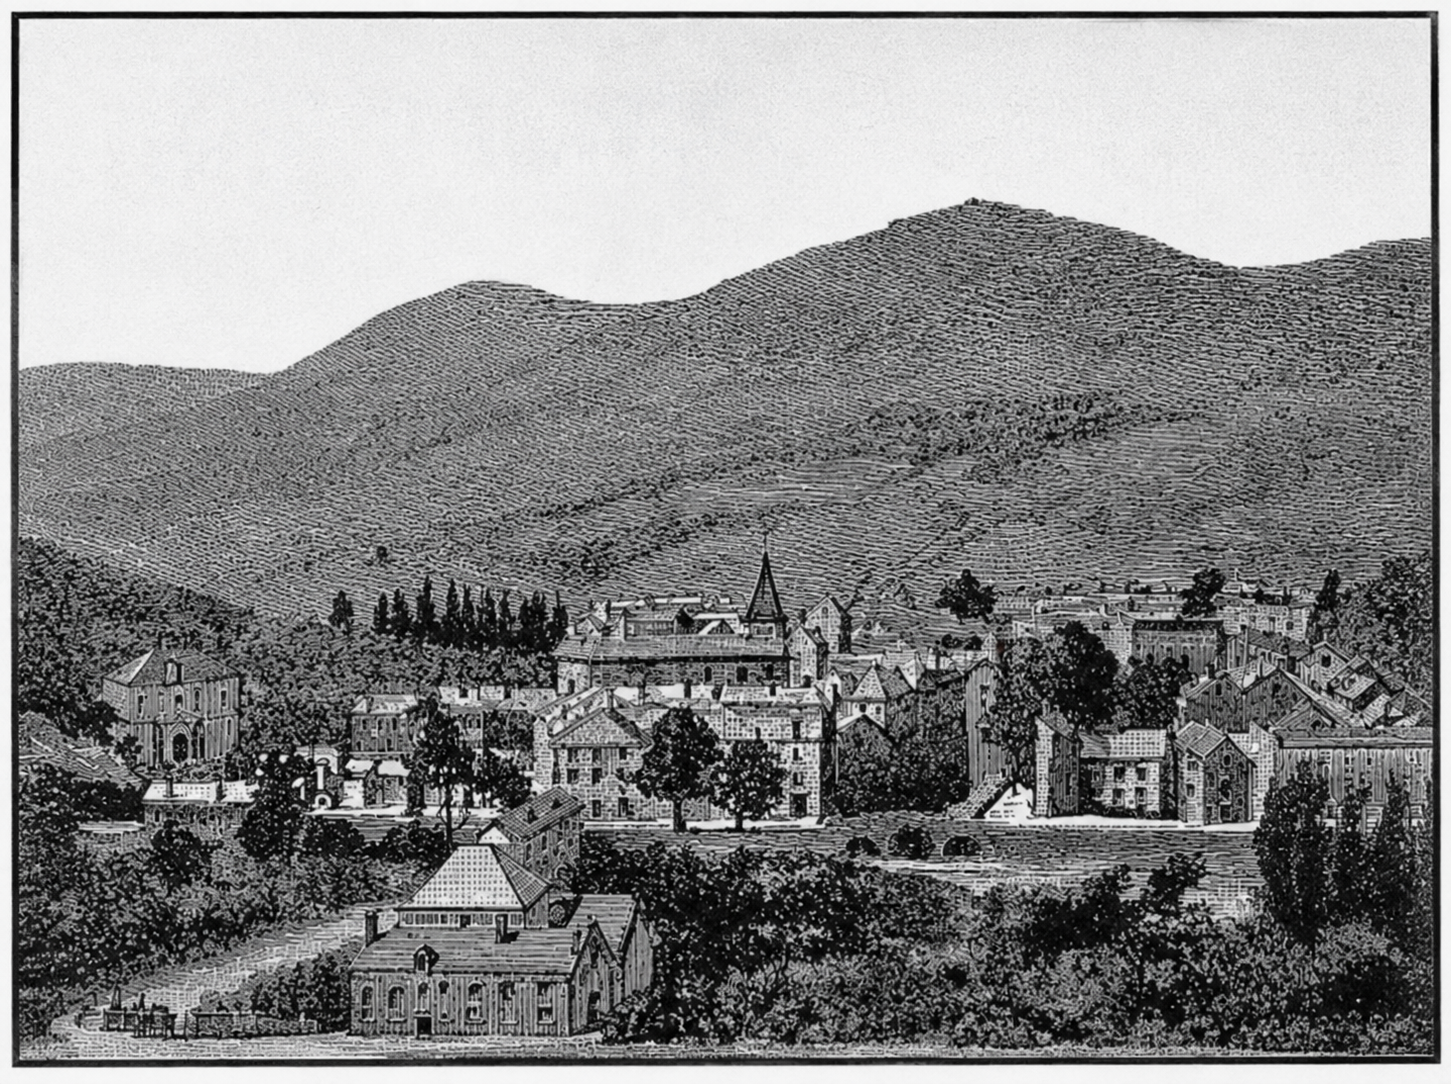
\includegraphics[width=0.60\textwidth]{imgs/132}\\
\emph{Meyrueis. 1890.}
\end{center}
